\documentclass[tikz,border=2pt]{standalone}
\usepackage{amsmath}
\usepackage{pgfplots}
\pgfplotsset{compat=1.18}
\usetikzlibrary{arrows.meta}
\begin{document}
% Poisson CGFs K(t) = lambda(e^t - 1) for lambda = 1 (X), 2 (Y) and 3 (X+Y, independent):
% the curves add pointwise, K_{X+Y} = K_X + K_Y, and each has slope lambda = mean at t = 0.
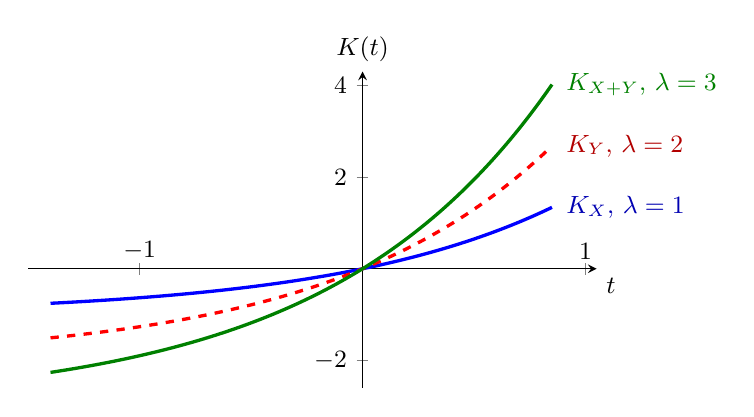
\begin{tikzpicture}[font=\small, >={Latex[length=2mm]}]
  \begin{axis}[
    axis lines=middle, xmin=-1.5, xmax=1.05, ymin=-2.6, ymax=4.3,
    xtick={-1,1}, ytick={-2,2,4}, xticklabel style={anchor=south, yshift=2pt},
    xlabel={$t$}, ylabel={$K(t)$},
    xlabel style={anchor=north west}, ylabel style={anchor=south},
    samples=100, smooth, width=8.8cm, height=5.6cm, clip=false]
    \addplot[blue, very thick, domain=-1.4:0.85] {exp(x)-1};
    \addplot[red, very thick, dashed, domain=-1.4:0.85] {2*(exp(x)-1)};
    \addplot[green!50!black, very thick, domain=-1.4:0.85] {3*(exp(x)-1)};
    \node[blue!70!black, anchor=west] at (axis cs:0.87,1.34) {$K_X$, $\lambda=1$};
    \node[red!70!black, anchor=west] at (axis cs:0.87,2.68) {$K_Y$, $\lambda=2$};
    \node[green!50!black, anchor=west] at (axis cs:0.87,4.02) {$K_{X+Y}$, $\lambda=3$};
  \end{axis}
\end{tikzpicture}
\end{document}
